\documentclass[a4paper,14pt, unknownkeysallowed]{bmstu}

\usepackage{cmap} % Улучшенный поиск русских слов в полученном pdf-файле
\usepackage[T2A]{fontenc} % Поддержка русских букв
\usepackage[utf8]{inputenc} % Кодировка utf8
\usepackage[english,russian]{babel} % Языки: русский, английский
\usepackage{enumitem}
\usepackage{graphics}
\usepackage{graphicx}
\usepackage{textcomp}
\usepackage{verbatim}
\usepackage{makeidx}
\usepackage{geometry}
\usepackage{float}
\usepackage{bm}
\usepackage{esint}
\usepackage{mathtools}
\usepackage{graphicx}
\usepackage{listings}
\usepackage{courier}
\usepackage{multirow}
\usepackage{graphicx}
\usepackage{xcolor}
\usepackage{titlesec}
\usepackage{csvsimple}

\usepackage{caption}
\captionsetup{labelsep=endash}
\usepackage{setspace}
\onehalfspacing % Полуторный интервал

% Для листинга кода:
\lstset{%
	language=c++,   					% выбор языка для подсветки
	basicstyle=\small\sffamily,			% размер и начертание шрифта для подсветки кода
	numbers=left,						% где поставить нумерацию строк (слева\справа)
	%numberstyle=,						% размер шрифта для номеров строк
	stepnumber=1,						% размер шага между двумя номерами строк
	numbersep=5pt,						% как далеко отстоят номера строк от подсвечиваемого кода
	frame=single,						% рисовать рамку вокруг кода
	tabsize=4,							% размер табуляции по умолчанию равен 4 пробелам
	captionpos=t,						% позиция заголовка вверху [t] или внизу [b]
	breaklines=true,
	breakatwhitespace=true,				% переносить строки только если есть пробел
	escapeinside={\#*}{*)},				% если нужно добавить комментарии в коде
	backgroundcolor=\color{white},
}

\author{Мансуров Владислав Михайлович}

\begin{document}
	\makereporttitle
	{Информатика и системы управления}
	{Программное обеспечение ЭВМ и информационные технологии}
	{Лабораторной работе}
	{Анализ Алгоритмов}
	{Динамическое программирование}
	{}
	{ИУ7-56Б}
	{Мансуров~В.~М.}
	{}

	\maketableofcontents
	\setcounter{page}{1}

\chapter*{Введение}
	\addcontentsline{toc}{chapter}{Введение}

	В данной лабораторной работе будет рассмотрено расстояние Левенштейна. Данное расстояние показывает минимальное количество операций (вставка, удаление, замены), которое необходимо для перевода одной строки в другую. Это расстояние помогает определить схожесть двух строк.

	Впервые задачу поставил в 1965 году советский математик Владимир Левенштейн при изучении последовательностей 0-1, впоследствии более общую задачу для произвольного алфавита связали с его именем.

	Расстояние Левенштейна применяется в теории информации и компьютерной лингвистике для:
	\begin{itemize}
    	\item исправления ошибок в слове(в поисковых системах, базах данных, при вводе текста, при автоматическом распознавании отсканированного текста или речи);
    	\item сравнения текстовых файлов утилитой diff;
    	\item для сравнения генов, хромосом и белков в биоинформатике.
    \end{itemize}

	Целью данной лабораторной работы является изучение и исследование особенностей задач динамического программирования на алгоритмах Левенштейна и Дамерау-Левенштейна.

	Для поставленной цели необходимо выполнить следующие задачи:
	\begin{enumerate}[label={\arabic*)}]
	    \item изучить расстояния Левенштейна и Дамерау-Левенштейна;
	    \item создать ПО, реализующее следующие алгоритмы:
	    \begin{itemize}
    	    \item нерекурсивный метод поиска расстояния Левенштейна;
    	    \item нерекурсивный метод поиска Дамерау-Левенштейна;
    	    \item рекурсивный метод поиска Дамерау-Левенштейна;
    	    \item  рекурсивный с кешированием метод поиска Дамерау-Левенштейна.
        \end{itemize}
        \item выбрать инструменты для замера процессорного времени выполнения реализаций алгоритмов;
        \item Провести анализ затрат работы программы по времени и по памяти, выяснить влияющие на них характеристики.
    \end{enumerate}

\chapter{Аналитическая часть}
	\section{Расстояние Левенштейна}

	Расстояние Левенштейна (редакционное расстояние, дистанция редактирования) --- метрика, измеряющая разность между двумя последовательностями символов.

	\noindentЦены операций могут зависеть от вида операций:
	\begin{enumerate}
       \item $w(a, b)$ --- цена замены символа $a$ на $b$, R (от англ. replace);
	    \item $w(\lambda, b)$ --- цена вставки символа $b$, I (от англ. insert);
	    \item $w(a, \lambda)$ --- цена удаления символа $a$, D (от англ. delete).
    \end{enumerate}

	\noindentБудем считать стоимость каждой вышеизложенной операции равной 1, то есть:
	\begin{itemize}
    	\item $w(a, b) = 1$, $a \neq b$;
    	\item $w(\lambda, b) = 1$;
    	\item $w(a, \lambda) = 1$.
    \end{itemize}

	\noindentВведем понятие совпадения символвов --- M ( от англ. match ). Его стоимость будет равна 0, то есть $w(a, a) = 0$.

	Расстояние Левенштейна между двумя строками $S_{1}$ и $S_{2}$, длинной M и N соответственно. Расстояние Левенштейна рассчитывается по рекуррентной формуле \ref{eq:D}:

	\begin{equation}
    	\label{eq:L}
    	D(i, j) =
    	\begin{cases}
    	0, &\text{i = 0, j = 0}\\
    	i, &\text{j = 0, i > 0}\\
    	j, &\text{i = 0, j > 0}\\
    	min \begin{cases}
    		D(i, j - 1) + 1\\
    		D(i - 1, j) + 1\\
    		D(i - 1, j - 1) +  m(S_{1}[i], S_{2}[i]) \\
    	    \end{cases}
    	&\text{i > 0, j > 0}
    	\end{cases}
    \end{equation}

    \begin{equation}
        \label{eq:m}
        m(a, b) = \begin{cases}
        0 &\text{если a = b,}\\
        1 &\text{иначе}
        \end{cases}.
    \end{equation}

    \subsection{Рекурсивный алгоритм нахождения расстояние Левенштейна}

    Рекурсивный алгоритм реализует формулу \ref{eq:L}, функция $D$ составлена таким образом, что:
    \begin{enumerate}
        \item  Для передачи из пустой строки в пустую требуется ноль операций;
        \item Для перевода из пустой строки в строку $a$ требуется $|a|$ операций;
        \item Для перевода из строки $a$ в пустую строку требуется $|a|$ операций;
        \item Для перевода из строки $a$ в строку $b$ требуется выполнить последовательно некоторое количество операций(удаление, вставка, замена) в некоторой последовательности. Последовательность поведения любых двух операций можно поменять, порядок поведения операций не имеет никакого значения. Пологая, что $a'$, $b'$ - строки $a$ и $b$ без последнего символа соответственно, цена преобразования из строки $a$ в строку $b$ может быть выражена как:
        \begin{itemize}
    	\item cумма цены преобразования строки $a$ в $b$ и цены проведения операции удаления, которая необходима для преобразования $a'$ в $a$;
    	\item cумма цены преобразования строки $a$ в $b$ и цены проведения операции вставки, которая необходима для преобразования $b'$ в $b$;
    	\item cумма цены преобразования из $a'$ в $b'$ и операции замены, предполагая, что $a'$ и $b'$ оканчиваются разные символы;
    	\item цена преобразования из $a'$ в $b'$ , предполагая, что $a$ и $b$ оканчиваются на один и тот же символ.
	\end{itemize}
    \end{enumerate}

    Минимальной ценой преобразования будет минимальное значение приведенных вариантов.

    \subsection{Рекурсивный алгоритм нахождения расстояния Левенштейна с кэшированием}

    Рекурсивная реализация алгоритма Левенштейна малоэффективна по времени при больших $i, j$, по причине проблемы повторных вычислений $D(i,j)$. Для оптимизации нахождения расстояния Левенштейна можно использовать матрицу в целях хранения соответствующих промежуточных значений. В таком случае алгоритм представляет собой рекурсивное заполнение матрицы $A_{|a|,|b|}$ значениями $D(i,j)$, такое хранение промежуточных данных можно назвать кэшом для рекурсивного алгоритма.

    \subsection{Нерекурсивный алгоритм нахождения расстояния Левенштейна}

    Рекурсивная реализация алгоритма Левенштейна с кэшированием малоэффективна по времени при больших $i, j$. Для оптимизации можно использовать итерационную реализацию заполнение матрицы промежуточными значениями $D(i,j)$.

    Однако матричный алгоритм является малоэффективным по памяти при больших $i, j$, т.к. множество промежуточных значений $D(i,j)$ хранится в памяти после их использования. Для оптимизации нахождения расстояния Левенштейна можно использовать кэш, т.е. пару строк, содержащюю значения $D(i,j)$, вычисленные в предыдущей итерации алгоритма и значения $D(i,j)$, вычисляемый в текущей итерации.

	\section{Расстояние Дамерау-Левенштейна}
	Расстояние Дамерау-Левенштейна(названо в честь учёных Фредерика Дамерау и Владимир Левенштейна) - это мера разницы двух строк символов, определяемая как минимальное количество операций вставки, удаления, замены и транспонзиций (перестановки двух соседних символов), необходимых для перевода одной строки в другую. Является модификацией расстояния Левенштейна, то есть к операциям добавляется операция транпонзиция T (от англ. transposition).

	Расстояние Дамерау-Левенштейна может быть вычисленно по рукурретной формуле:

	\begin{equation}
    	\label{eq:DL}
    	D(i, j) = \begin{cases}
    	0  \qquad\qquad\qquad\qquad\qquad\qquad\qquad\qquad\qquad,j = 0, i = 0\\
    	i  \qquad\qquad\qquad\qquad\qquad\qquad\qquad\qquad\qquad,j = 0, i > 0\\
    	j  \qquad\qquad\qquad\qquad\qquad\qquad\qquad\qquad\qquad,j > 0, i = 0\\
    	min \begin{cases}
    		D(i, j - 1) + 1\\
    		D(i - 1, j) + 1\\
    		D(i - 1, j - 1) + m(S_{1}[i], S_{2}[i]) \\
    		D(i - 2, j - 2) + m(S_{1}[i], S_{2}[i]) \\
    	\end{cases}
    	\begin{aligned}
    		& , \text{если i > 1, j > 1} \\
    		& , S_{1}[i] = S_{2}[j - 1]  \\
    		& , S_{1}[j] =  S_{2}[i - 1] \\
    	\end{aligned}\\
    	min \begin{cases}
    		D(i, j - 1) + 1\\
    		D(i - 1, j) + 1 & \;\; \text{,иначе}\\
    		D(i - 1, j - 1) + m(S_{1}[i], S_{2}[i]) \\
    	\end{cases}
	\end{cases}
\end{equation}

\section{Вывод}

В данном разделе были рассмотрены алгоритмы динамического программирования - алгоритмы нахождения расстояния Левенштейна и Дамерау-Левенштейна, формулы которых задаются реккурентно, а следовательно, данные алгоритмы могут быть реализованы рекурсивно и итерационно. На вход алгоритмам поступают две строки, которые могут содержать как русские, так и английские буквы, также будет предусмотрен ввод пустых строк.

\chapter{Конструкторская часть}

В данном разделе будут приведены схемы алгоритмов нахождения расстояний Левенштейна и Дамерау-Левенштейна, приведено описанию используемых типов данных, оценки памяти, а также описана структура ПО.

\section{Разработка алгоритмов}

На вход алгоритмов подаются строки $S_1$ и $S_2$

На рисунке \ref{fig:Liter} представлен схема алгоритма поиска расстояния Левенштейна.

На рисунках \ref{fig:DLiter} - \ref{fig:DLrechash2} представлены схемы алгоритмов поиска Дамерау-Левенштейна.

\begin{figure}[h]
	\centering
	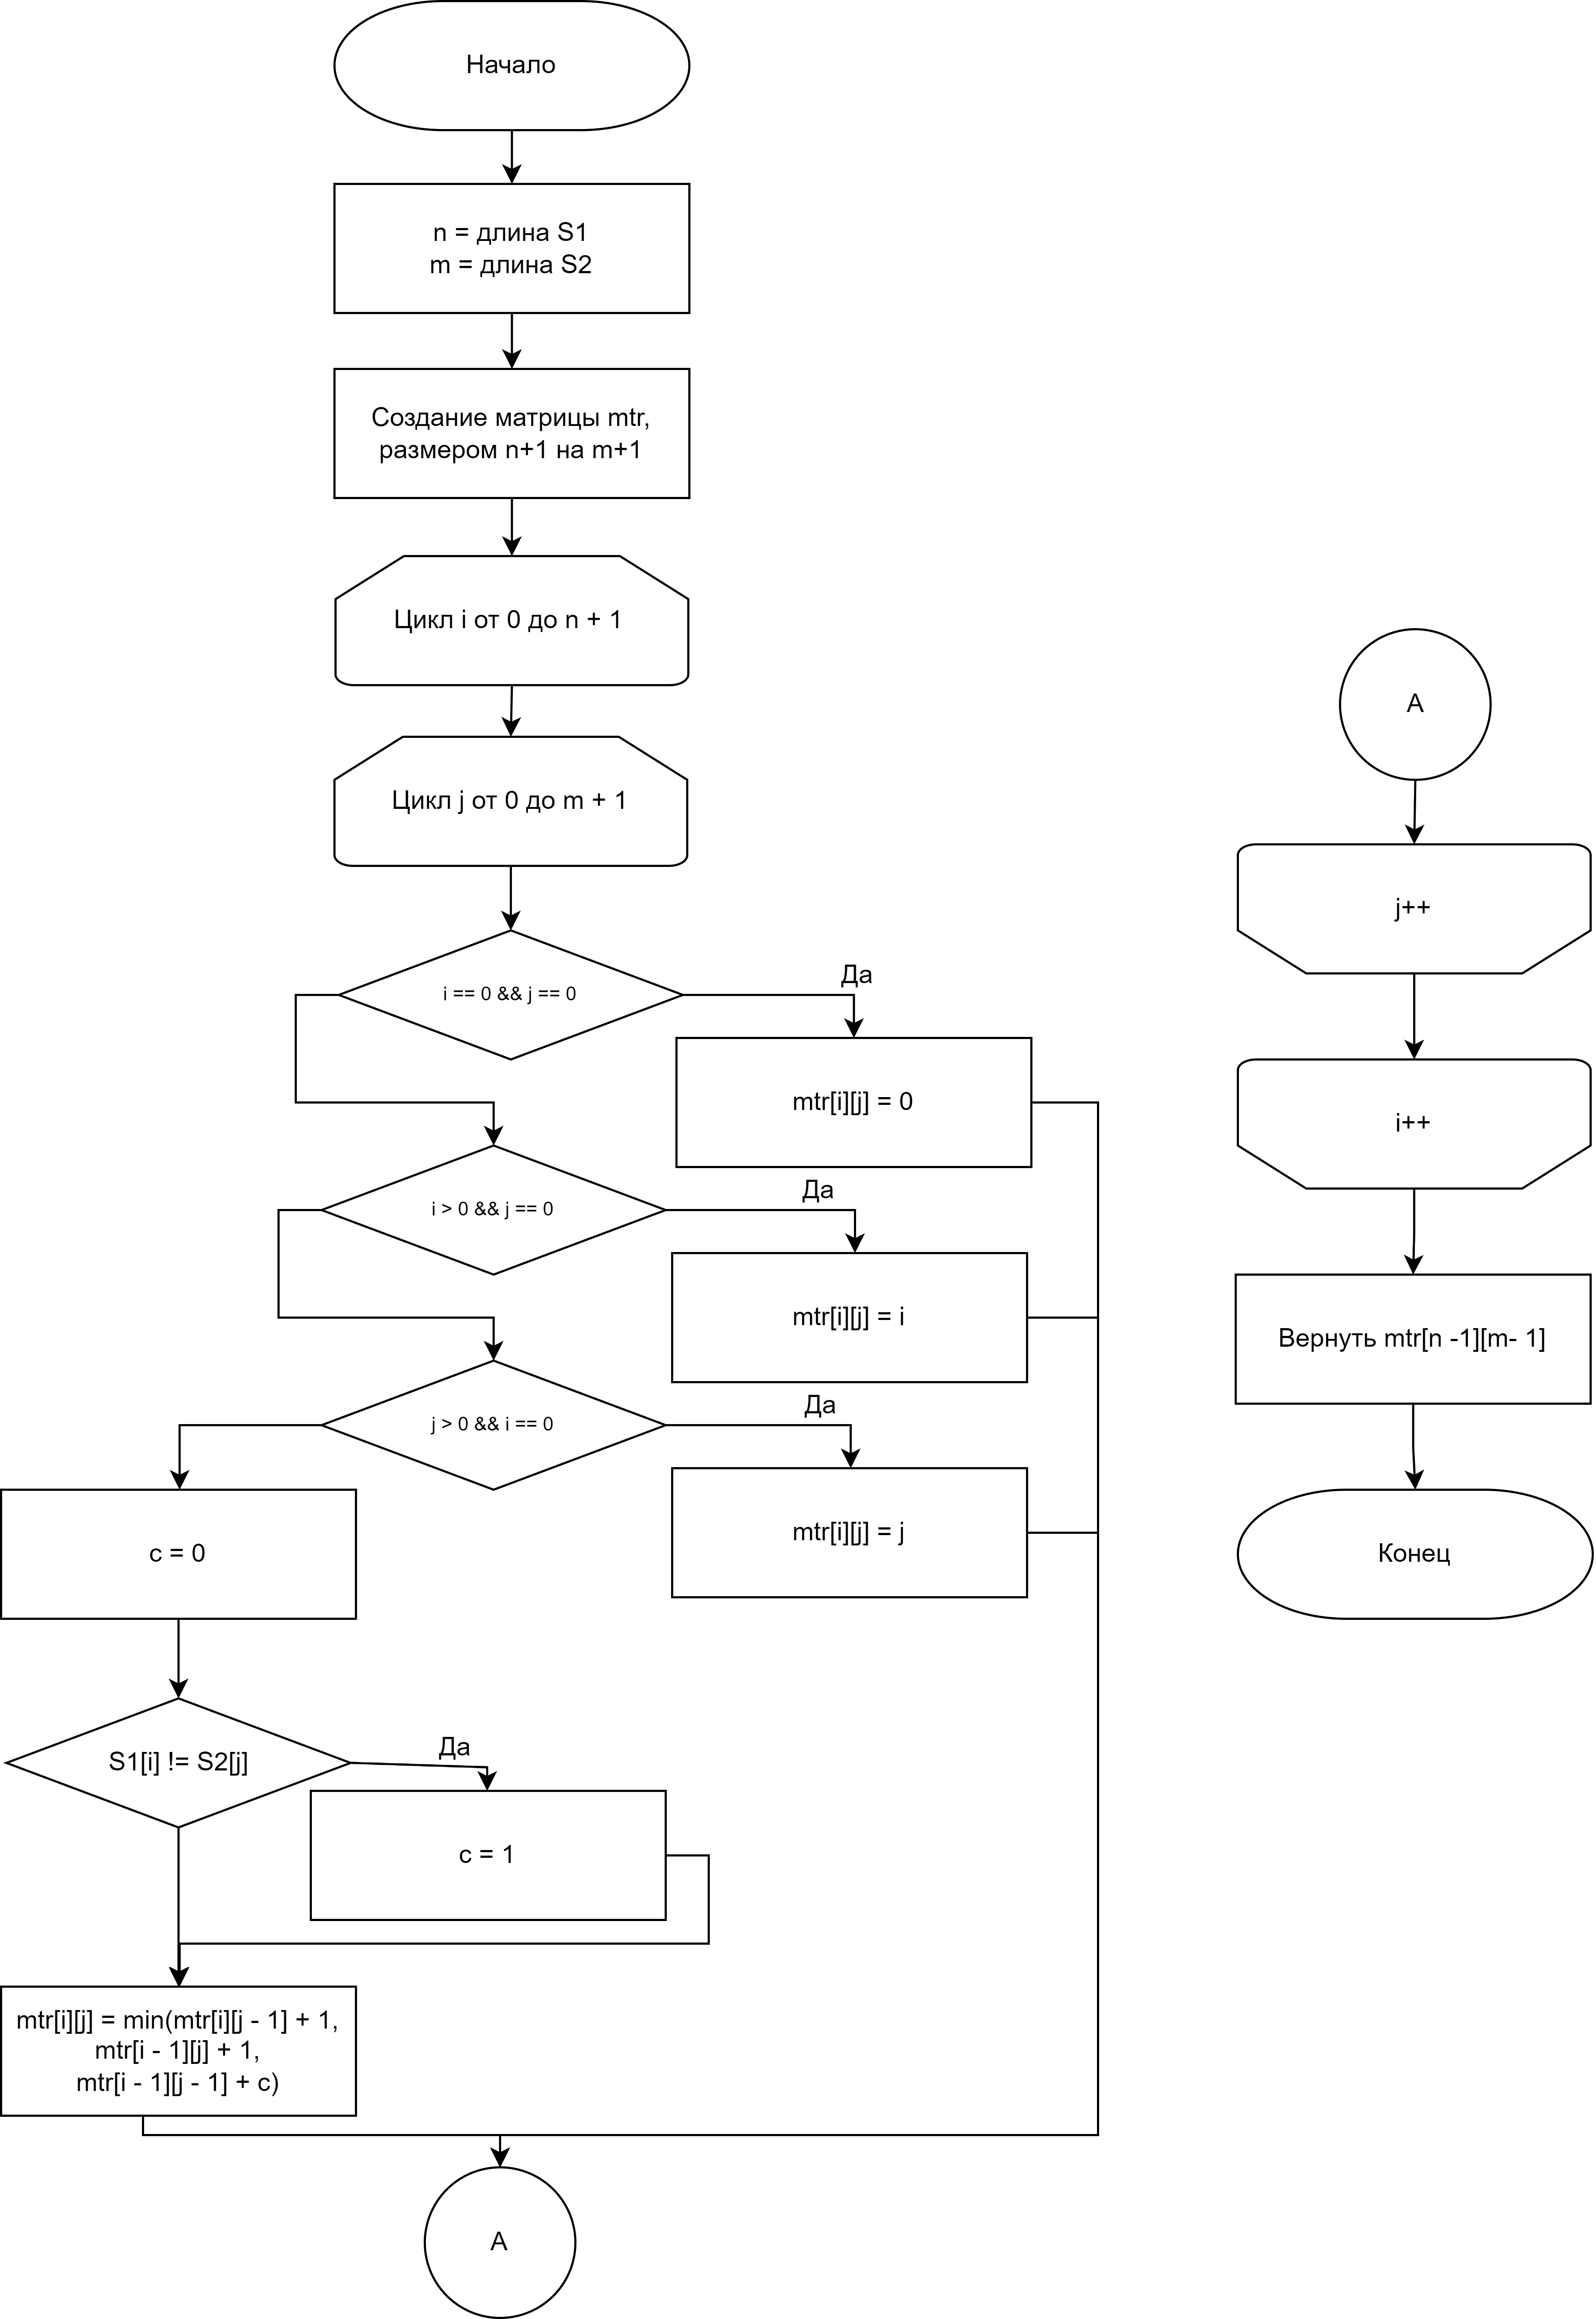
\includegraphics[height=0.8\textheight]{img/levmatr.png}
	\caption{Схема нерекурсивного алгоритма нахождения расстояния Левенштейна}
	\label{fig:Liter}
\end{figure}

\clearpage

\begin{figure}[h]
	\centering
	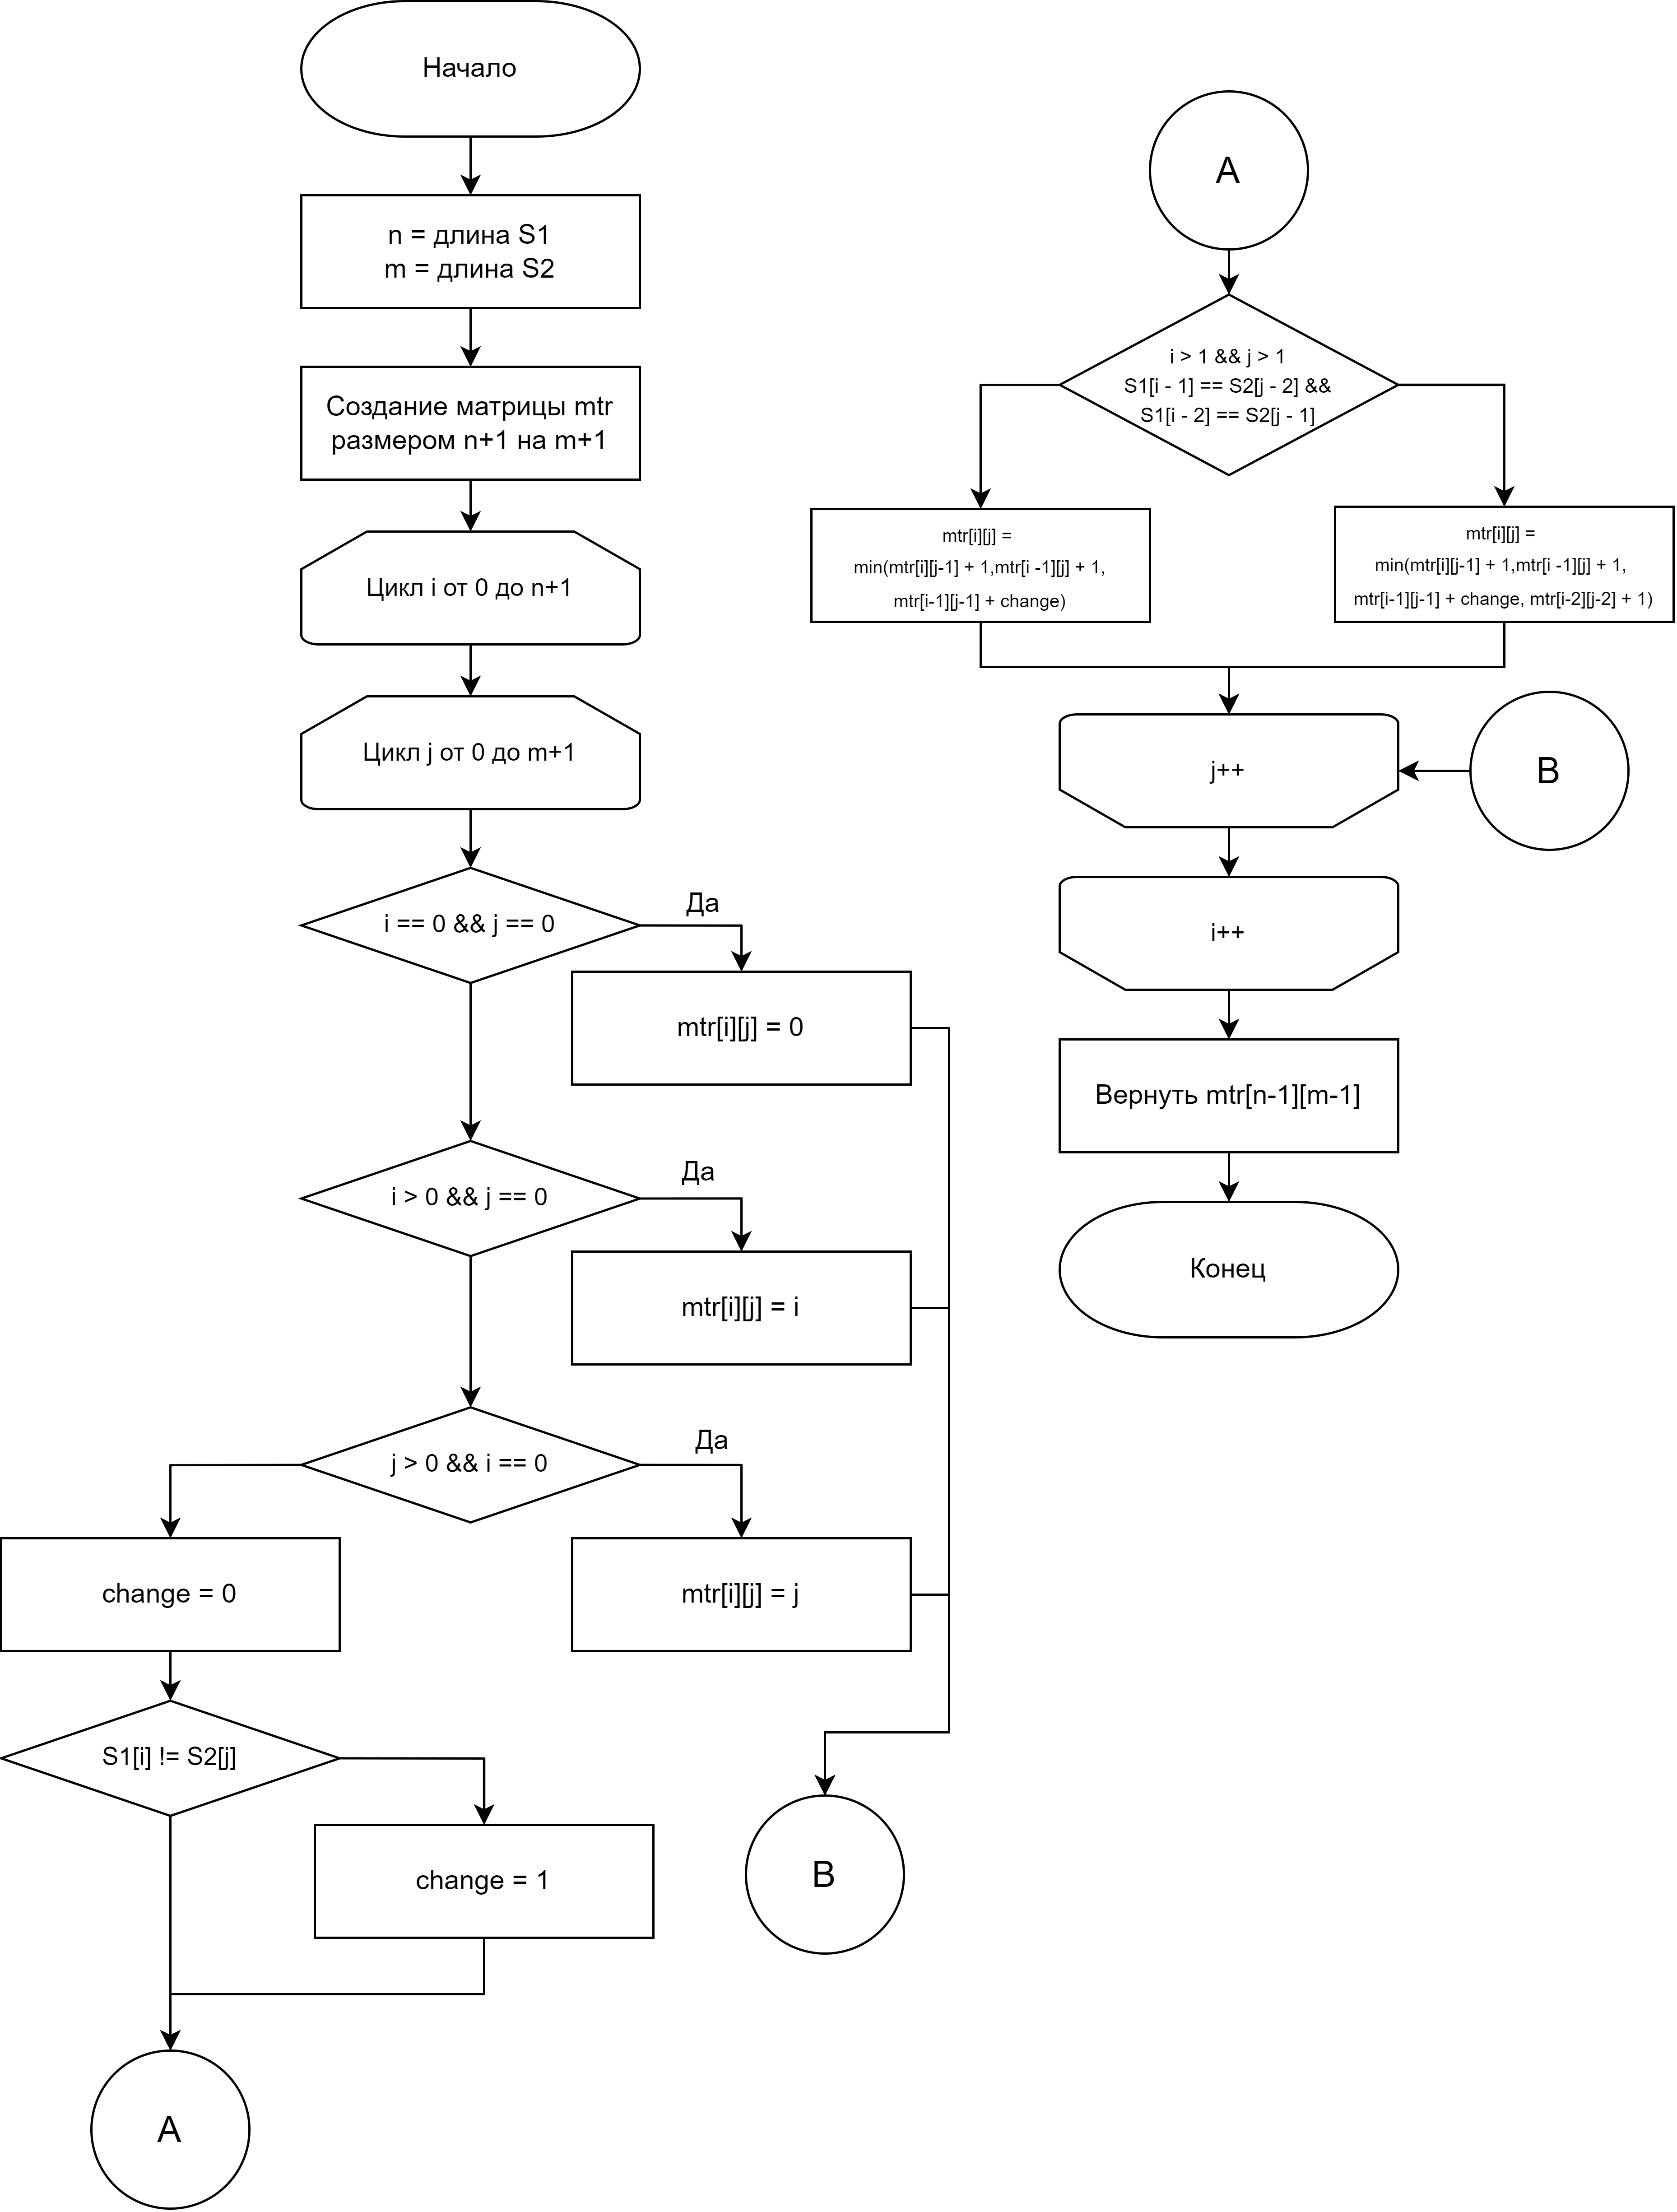
\includegraphics[height=0.8\textheight]{img/dliter.png}
	\caption{Схема нерекурсивного алгоритма нахождения расстояния Дамерау-Левенштейна}
	\label{fig:DLiter}
\end{figure}

\clearpage

\begin{figure}[h]
	\centering
	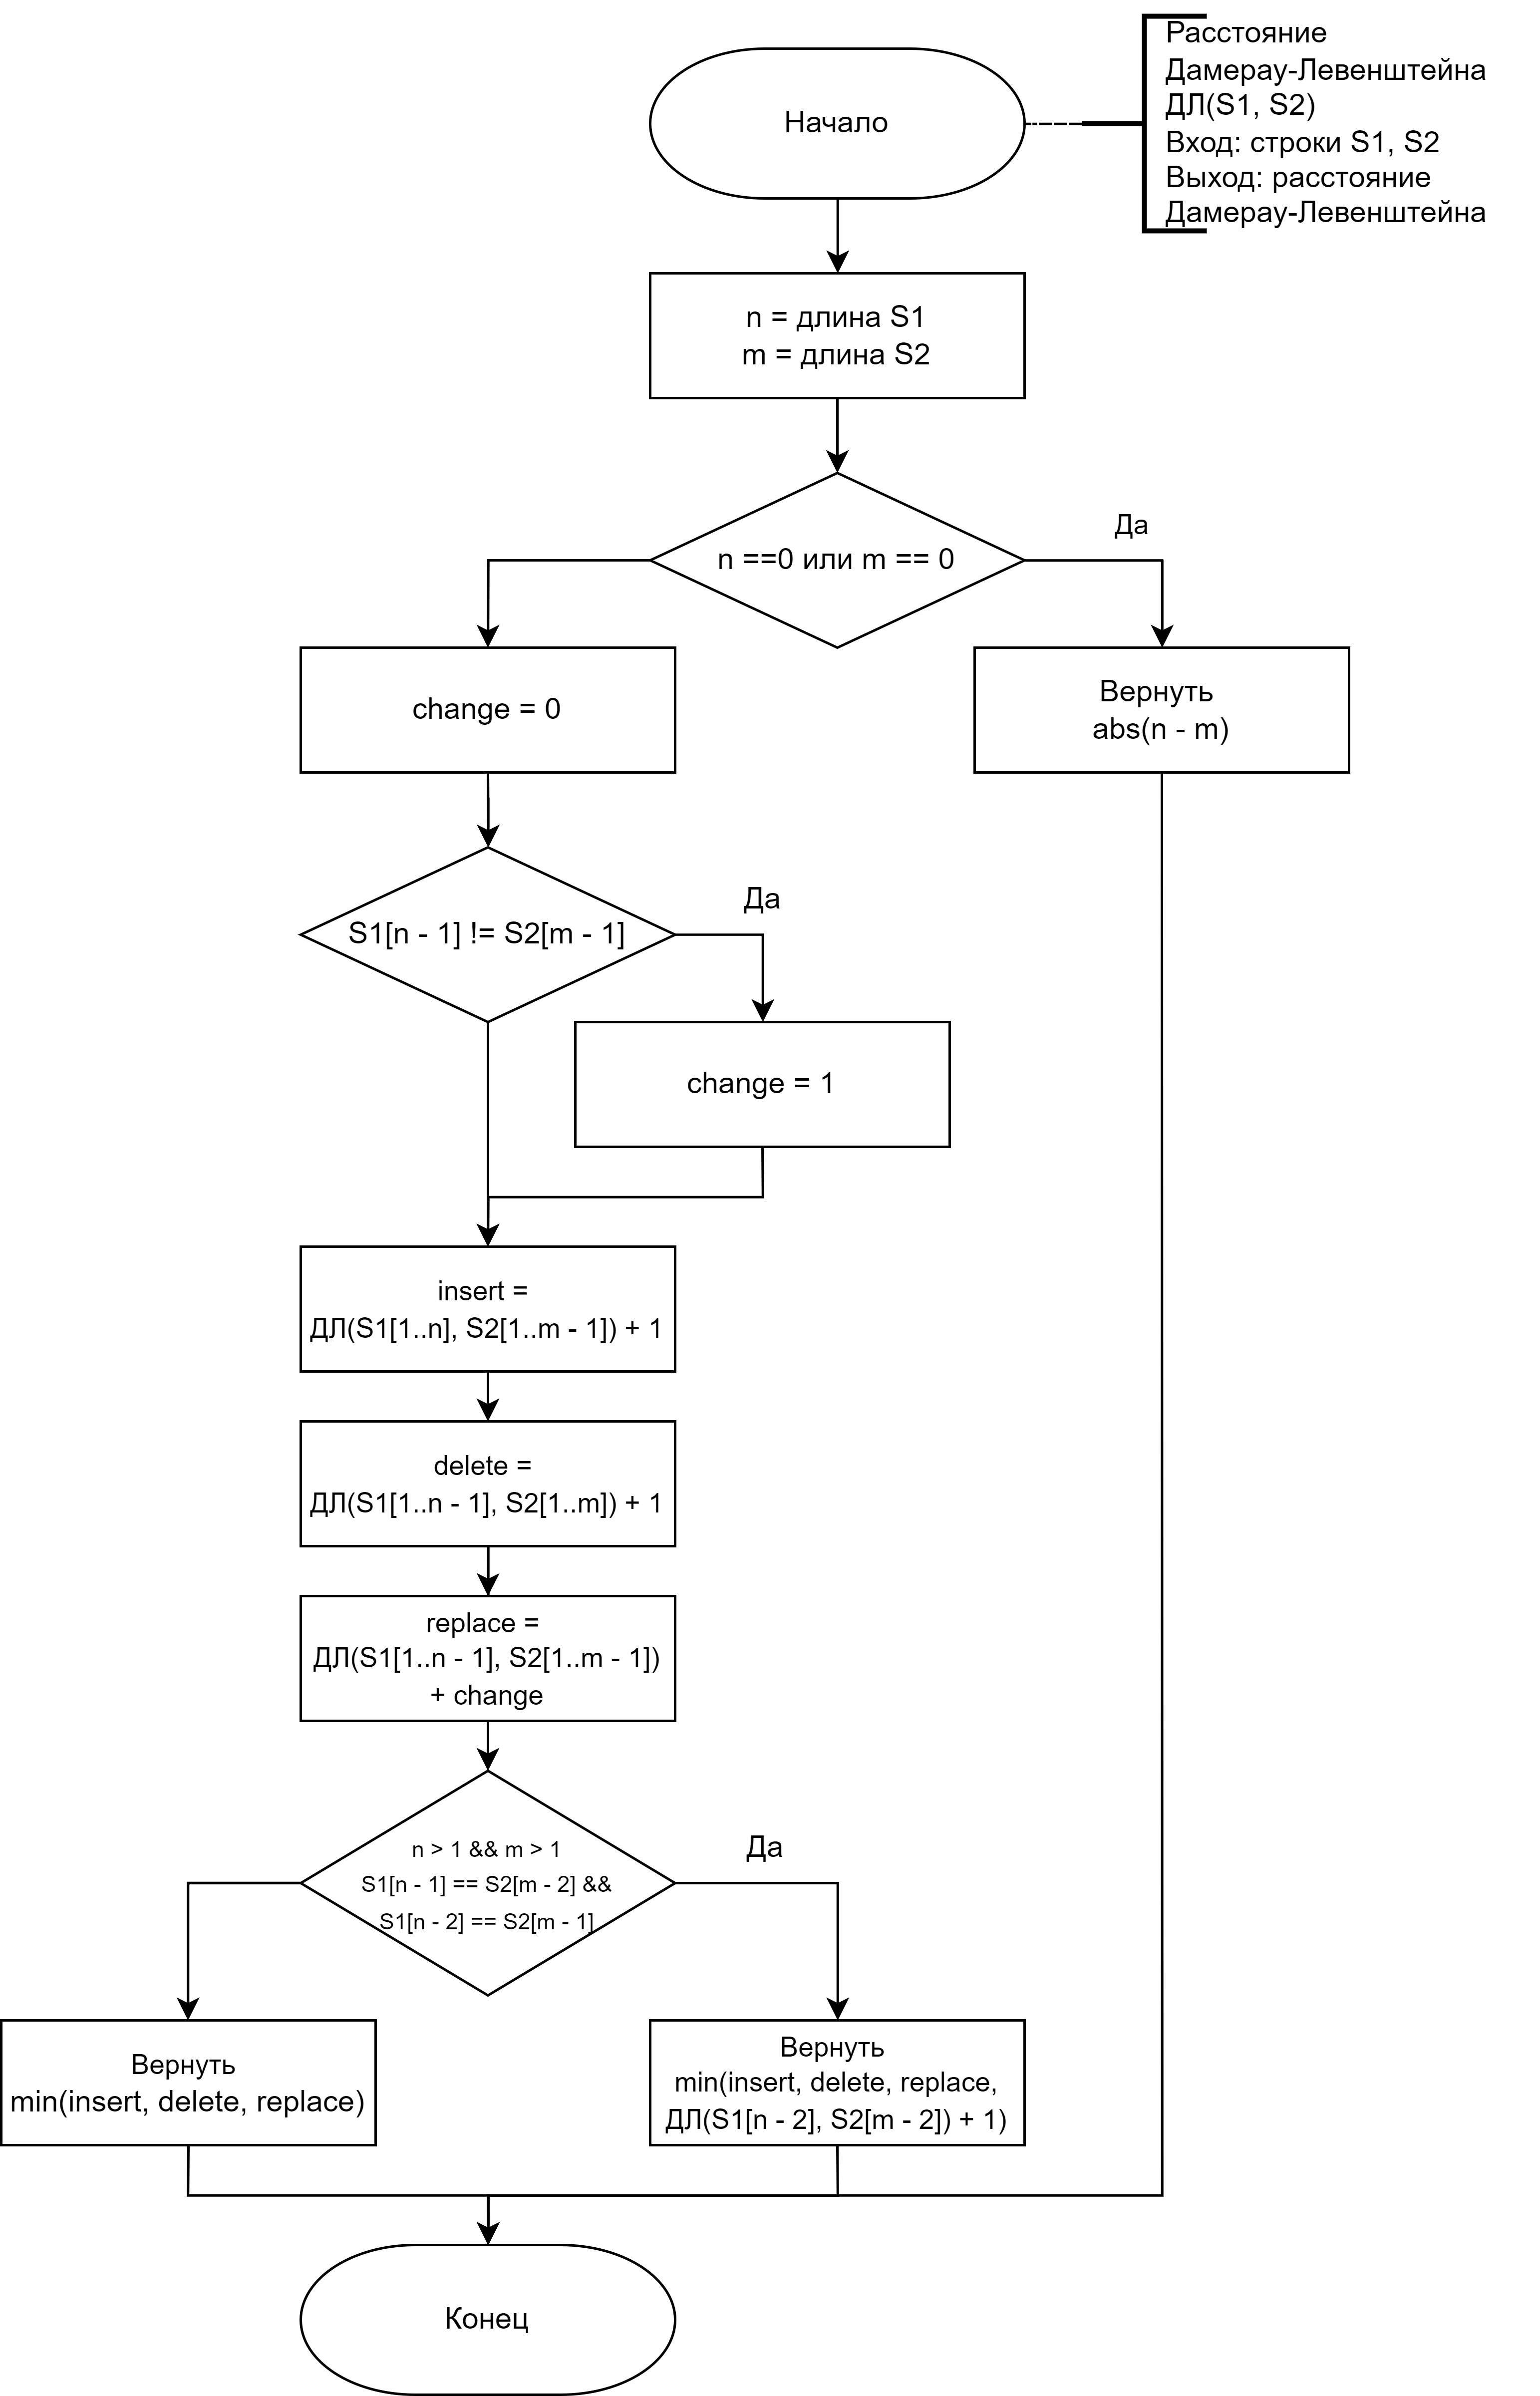
\includegraphics[height=0.8\textheight]{img/dlrec.png}
	\caption{Схема рекурсивного алгоритма нахождения расстояния Дамерау-Левенштейна}
	\label{fig:DLrec}
\end{figure}

\clearpage

\begin{figure}[h]
	\centering
	
\includegraphics[height=0.6\textheight]{img/dlrechash-1.png}
	\caption{Схема рекурсивного алгоритма нахождения расстояния Дамерау-Левенштейна с кэшированием}
	\label{fig:DLrechash1}
\end{figure}

\clearpage

\begin{figure}[h]
	\centering
	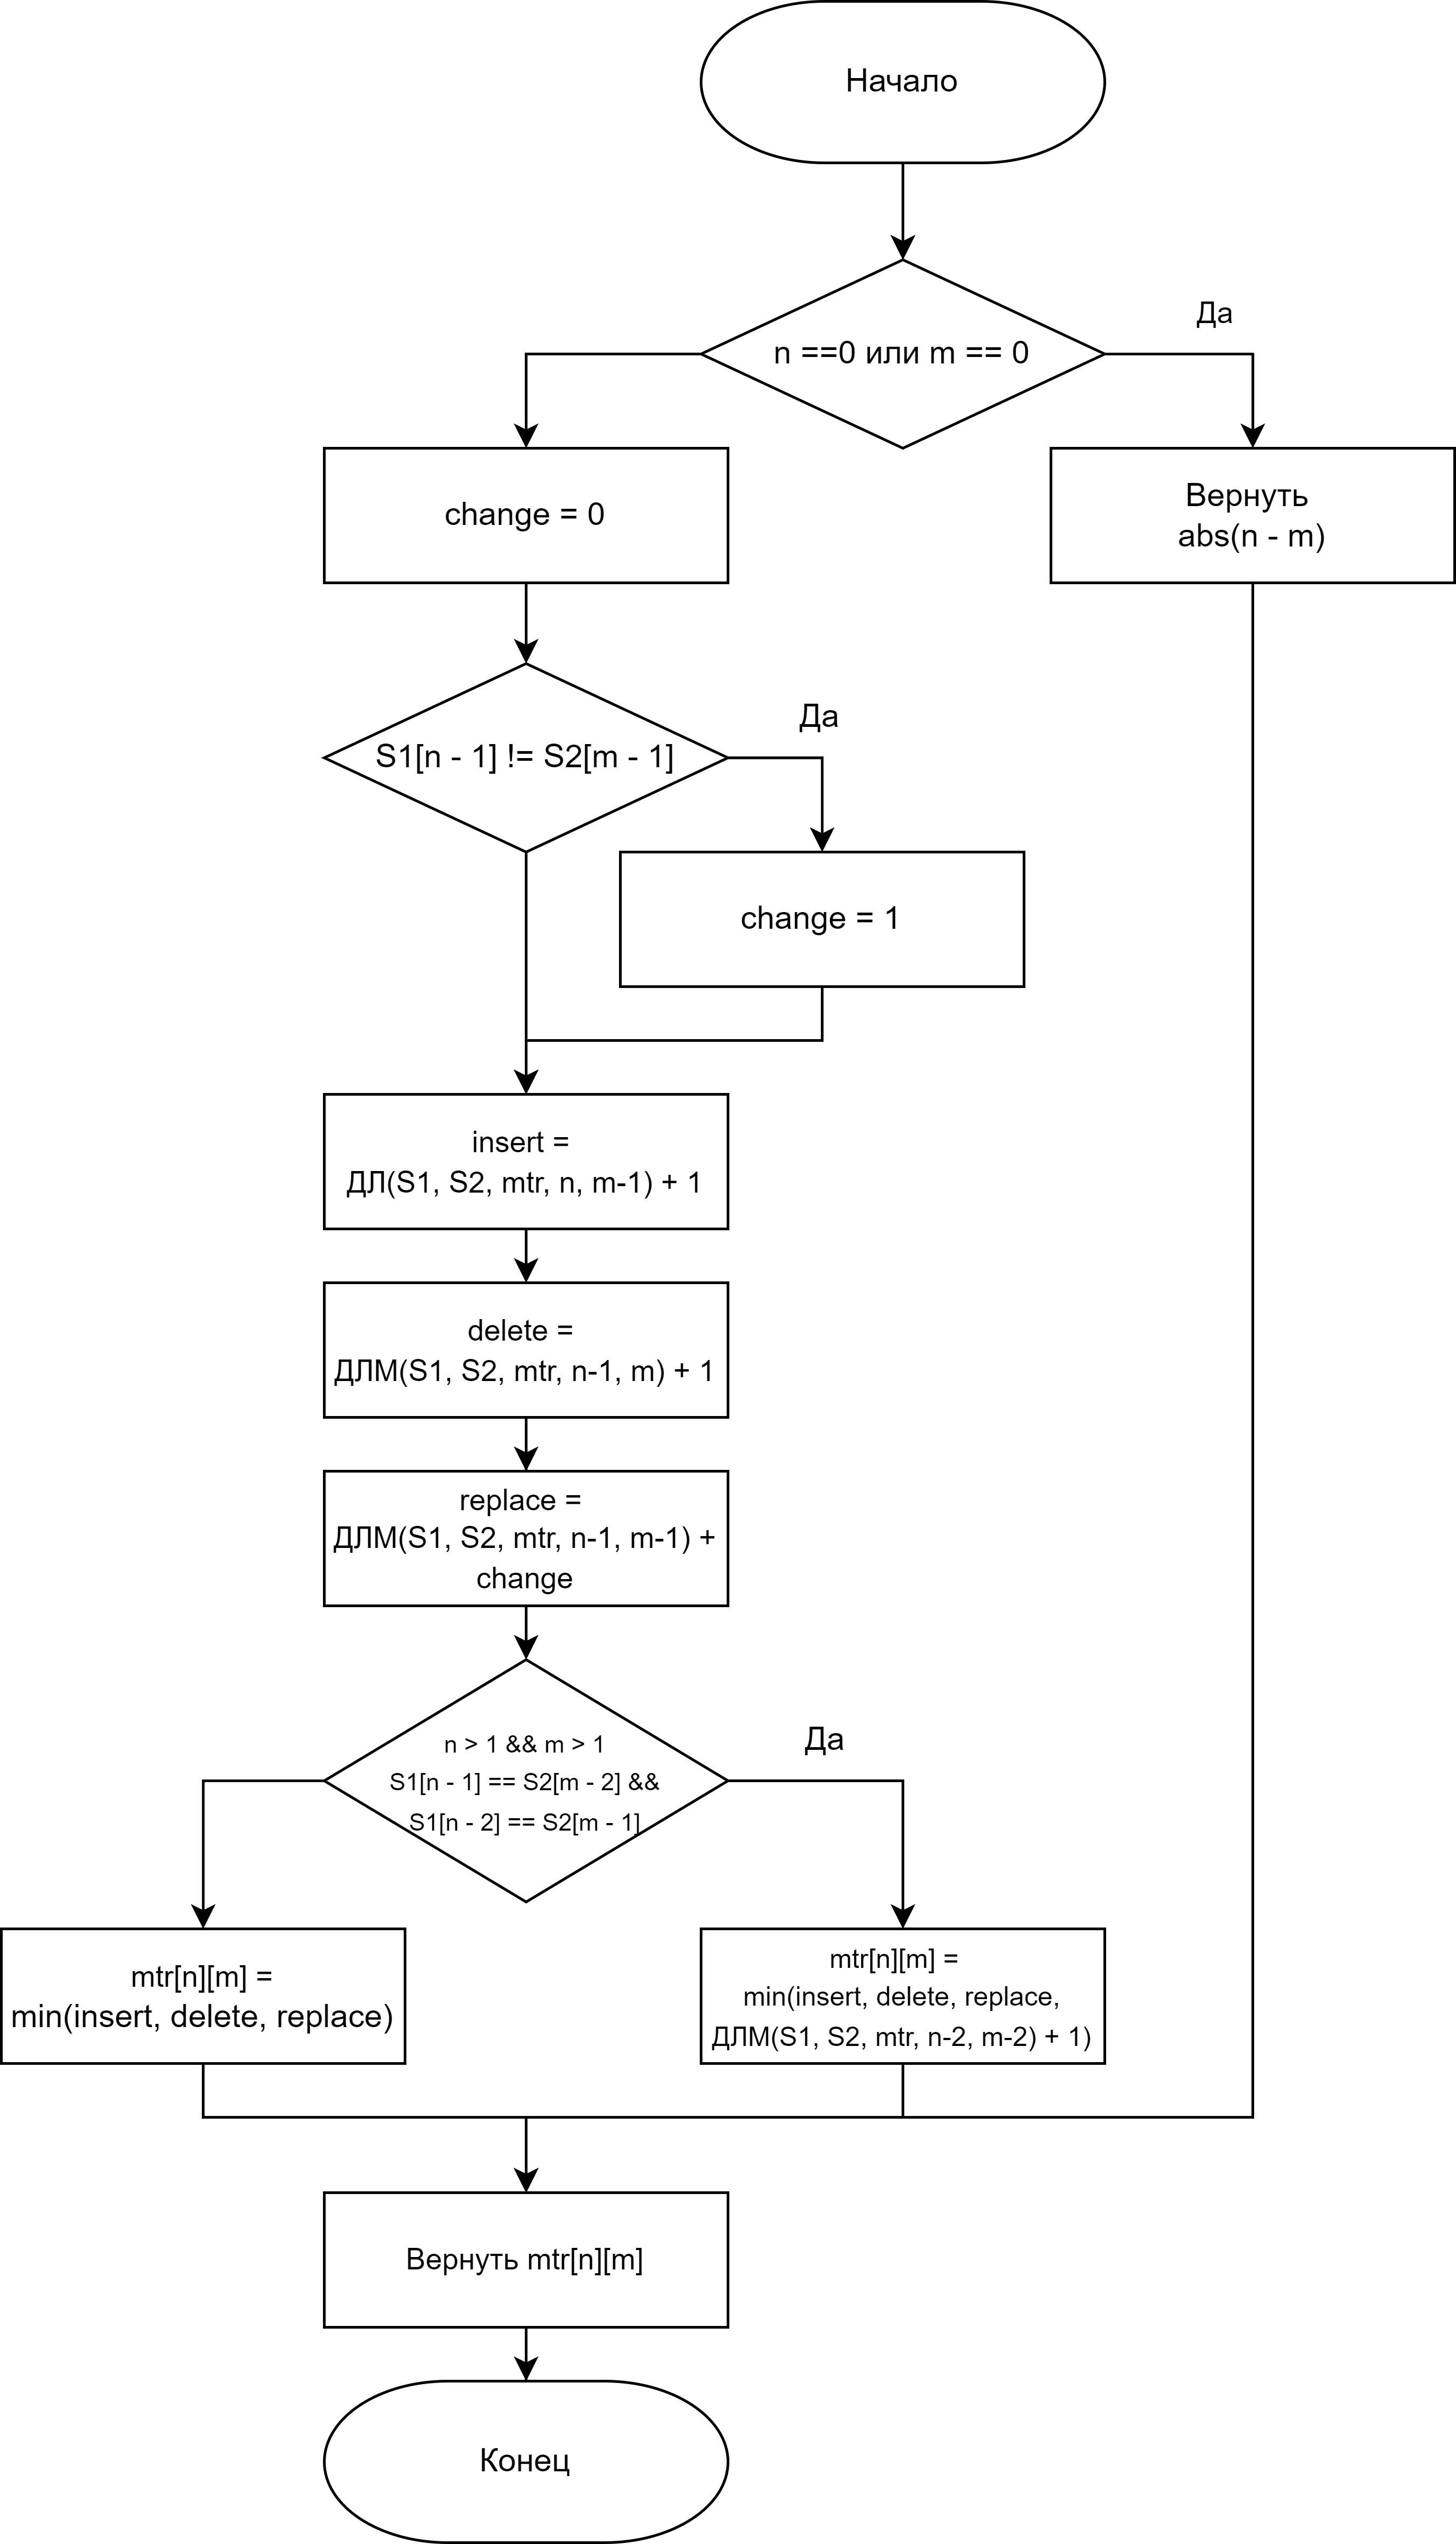
\includegraphics[height=0.8\textheight]{img/dlrechash-2.png}
	\caption{Схема алгоритма рекурсивного заполнения матрицы расстоянием Дамерау-Левенштейна}
	\label{fig:DLrechash2}
\end{figure}

\clearpage

\section{Описание используемых типов данных}

При реализации алгоритмов будут использованы следующие структуры данных:

\begin{itemize}
	\item строка - массив типа $char$ размером длины строки;
	\item длина строки - целое число типа $int$;
	\item матрица - двумерный массив типа $int$.
\end{itemize}

\section{Вывод}

В данном разделе на основе теоретических данных были построены схемы
требуемых алгоритмов, выбраны используемые типы данных.

\chapter{Технологическая часть}

В данном разделе будут приведены требования к программному обеспечению, средства реализации, листинг кода и функциональные тесты.

\section{Требования к программному обеспечению}

К программе предъявлены ряд требований:

\begin{itemize}
	\item входные данные - две строки на русском или английском языке в любом
регистре;
    \item На выходе — результат выполнения каждого из вышеуказанных алгоритмов.
\end{itemize}

\section{Средства реализации}

В качестве языка программирования для реализации данной лабораторной работы был выбран язык $C++$. Данный выбор обусловлен тем,
что я имею некоторый опыт разработки на нем, а так же наличием у языка
встроенны библиотеки измерения процессорного времени и тип данных работающий как с кириллицей, так и с латиницей -- $std::wstring$.


\section{Сведения о модулях программы}

Данная программа разбита на следующие модули:

\begin{itemize}
	\item \texttt{main.cpp} -- Файл, содержащий точку входа в программу. В нем происходит
общение с пользователем и вызов алгоритмов;
    \item \texttt{algorithms.cpp} –- Файл содержит функции поиска расстояния Левенштейна и Дамерау-Левенштейна.
    \item \texttt{allocate.cpp} –- Файл содержит функции динамического выделения и очищения памяти для матрицы.
    \item \texttt{print\_mtr\_lev.cpp} -- Файл содержит функции вывода матрицы для итерационных методов поиска расстояния Левенштейна и Дамеру-Левештейна, включая строки.
    \item \texttt{cpu\_time.cpp} –- Файл содержит функции, замеряющее процессорное время алгоритмов поиска расстояния Левеншьейна и Дамерау-Левенштейна.
    \item \texttt{memory.cpp} –- Файл содержит функции, замеряющее память итерационного и рекурсивного алгоритмов поиска расстояния Левенштейна.
\end{itemize}

\begin{lstlisting}[label=lst:lev_mtr,caption=Функция нахождения расстояния Левенштейна с использованием матрицы]
int lev_mtr(wstring &str1, wstring &str2, bool print )
{
    size_t n = str1.length();
    size_t m = str2.length();
    int **mtr = malloc_mtr(n + 1, m + 1);
    int res = 0;

    for (int i = 0; i <= n; i++)
        for (int j = 0; j <= m; j++)
            if (i == 0 && j == 0)
                mtr[i][j] = 0;
            else if (i > 0 && j == 0)
                mtr[i][j] = i;
            else if (j > 0 && i == 0)
                mtr[i][j] = j;
            else {
                int change = 0;
                if (str1[i - 1] != str2[j - 1])
                    change = 1;

                mtr[i][j] = std::min(mtr[i][j - 1] + 1,
                                     std::min(mtr[i - 1][j] + 1,
                                              mtr[i - 1][j - 1] + change));
            }

    if (print)
        print_mtr_lev(str1, str2, mtr, n, m);
    res = mtr[n][m];
    free_mtr(mtr, n);

    return res;
}
\end{lstlisting}

\clearpage

\begin{lstlisting}[label=lst:dameray_lev_rec,caption=Функция нахождения расстояния Дамерау-Левенштейна с использованием матрицы]
int dameray_lev_mtr(wstring &str1, wstring &str2, bool print)
{
    size_t n = str1.length();
    size_t m = str2.length();
    int **mtr = malloc_mtr(n + 1, m + 1);
    int res = 0;

    for (int i = 0; i <= n; i++)
        for (int j = 0; j <= m; j++) {
            if (i == 0 && j == 0)
                mtr[i][j] = 0;
            else if (i > 0 && j == 0)
                mtr[i][j] = i;
            else if (j > 0 && i == 0)
                mtr[i][j] = j;
            else {
                int change = 0;
                if (str1[i - 1] != str2[j - 1])
                    change = 1;

                mtr[i][j] = min(mtr[i][j - 1] + 1,
                                min(mtr[i - 1][j] + 1,
                                    mtr[i - 1][j - 1] + change));

                if (i > 1 && j > 1 &&
                    str1[i - 1] == str2[j - 2] &&
                    str1[i - 2] == str2[j - 1])
                    mtr[i][j] = min(mtr[i][j], mtr[i - 2][j - 2] + 1);
            }
        }

    if (print)
        print_mtr_lev(str1, str2, mtr, n, m);
    res = mtr[n][m];
    free_mtr(mtr, n);

    return res;
}
\end{lstlisting}

\clearpage

\begin{lstlisting}[label=lst:dameray_lev_mtr,caption=Функция нахождения расстояния Дамерау-Левенштейна рекурсивно]
int dameray_lev_rec_t(wstring &str1, wstring &str2, size_t n, size_t m) {
    if (n == 0)
        return m;
    if (m == 0)
        return n;

    int change = 0;
    int res = 0;
    if (str1[n - 1] != str2[m - 1])
        change = 1;

    res = min(dameray_lev_rec_t(str1, str2, n, m - 1) + 1,
              min(dameray_lev_rec_t(str1, str2, n - 1, m) + 1,
                  dameray_lev_rec_t(str1, str2, n - 1, m - 1) + change));

    if (n > 1 && m > 1 &&
        str1[n - 1] == str2[m - 2] &&
        str1[n - 2] == str2[m - 1])
        res = std::min(res, dameray_lev_rec_t(str1, str2, n - 2, m - 2) + 1);
    return res;
}

int dameray_lev_rec(wstring &str1, wstring &str2)
{
    return dameray_lev_rec_t(str1, str2, str1.length(), str2.length());
}
\end{lstlisting}

\clearpage

\begin{lstlisting}[label=lst:dameray_lev_rec_hash,caption=Функция нахождения расстояния Дамерау-Левенштейна рекурсивно c кэшированием]
int dameray_lev_rec_hash_t(wstring &str1, wstring &str2, int **mtr, size_t n, size_t m)
{
    if (n == 0)
        return mtr[n][m] = m;
    if (m == 0)
        return mtr[n][m] = n;
    int change = 0;
    if (str1[n - 1] != str2[m - 1])
        change = 1;
    mtr[n][m] = min(dameray_lev_rec_hash_t(str1, str2, mtr, n, m - 1) + 1,
                    min(dameray_lev_rec_hash_t(str1, str2, mtr, n - 1, m) + 1,
                        dameray_lev_rec_hash_t(str1, str2, mtr, n - 1, m - 1) + change));
    if (n > 1 && m > 1 &&
        str1[n - 1] == str2[m - 2] &&
        str1[n - 2] == str2[m - 1])
        mtr[n][m] = min(mtr[n][m], dameray_lev_rec_hash_t(str1, str2, mtr, n - 2, m - 2) + 1);
    return mtr[n][m];
}

int dameray_lev_rec_hash(wstring &str1, wstring &str2, bool print)
{
    size_t n = str1.length();
    size_t m = str2.length();
    int **mtr = malloc_mtr(n + 1, m + 1);
    for (int i = 0; i <= n; i++)
        for (int j = 0; j <= m; j++) {
                mtr[i][j] = -1;
        }
    int res = dameray_lev_rec_hash_t(str1, str2, mtr, n, m);
    if (print)
        print_mtr_lev(str1, str2, mtr, n, m);
    free_mtr(mtr, n);
    return res;
}
\end{lstlisting}

\clearpage

\begin{lstlisting}[label=lst:allocate_mtr,caption=Функции динамического выделения и очищения памяти под матрицу]
void free_mtr(int **mtr, std::size_t n) {
    if (mtr != nullptr)
    {
        for (std::size_t i = 0; i < n; i++)
            if (mtr[i] != nullptr)
                free(mtr[i]);
        free(mtr);
    }
}

int **malloc_mtr(std::size_t n, std::size_t m)
{
    if (n == 0)
        return nullptr;

    int **mtr = static_cast<int **>(malloc(n * sizeof(int *)));
    if (mtr != nullptr)
        for (std::size_t i = 0; mtr[i] != nullptr && i < n; i++) {
            mtr[i] = static_cast<int *>(malloc(m * sizeof(int)));
            if (mtr[i] == nullptr)
                free_mtr(mtr, n);
        }

    return mtr;
}
\end{lstlisting}

\clearpage

\begin{lstlisting}[label=lst:print_mtr,caption=Функции вывода матрицы для алгоритмов поиска расстояния Левенштейна и Дамерау-Левенштейна]
void print_mtr_lev(std::wstring str1, std::wstring str2,
                   int **mtr, std::size_t n, std::size_t m)
{
    for(std::size_t i = 0; i <= n + 1; i++)
    {
        for(std::size_t j = 0; j <= m + 1; j++)
        {
            if (i == 0 && j == 0)
                std::wcout << "  ";
            else if (i == 0)
                if (j == 1)
                    std::wcout << "- ";
                else
                    std::wcout << str2[j - 2] << " ";
            else if (j == 0)
                if (i == 1)
                    std::wcout << "- ";
                else
                    std::wcout << str1[i - 2] << " ";
            else
                std::wcout << mtr[i - 1][j - 1] << " ";
        }
        std::wcout << std::endl;
    }
}
\end{lstlisting}

\clearpage

\section{Функциональные тесты}

В таблице \ref{tbl:func_tests} приведены функциональные тесты для алгоритмов вычисления расстояния Левенштейна и Дамерау—Левенштейна. Все тесты пройдены успешно.

\begin{table}[ht]
	\small
	\begin{center}
		\caption{Функциональные тесты}
		\label{tbl:func_tests}
		\begin{tabular}{|c|c|c|c|c|c|}
			\hline
			&
			& \multicolumn{1}{c|}{\bfseries Левенштейн}
			& \multicolumn{3}{c|}{\bfseries Дамерау-Левенштейн} \\ \cline{3-6}

			\bfseries Строка 1 & \bfseries Строка 2 & \bfseries Итеративный & \bfseries Итеративный

			& \multicolumn{2}{c|}{\bfseries Рекурсивный} \\ \cline{5-6}
			& & & & \bfseries Без кэша & \bfseries С кэшом \\
			\hline
			a & b & 1 & 1 & 1 & 1 \\
			\hline
			a & a & 0 & 0 & 0 & 0 \\
			\hline
			кот & скат & 2 & 2 & 2 & 2 \\
			\hline
			друзья & рдузия & 3 & 2 & 2 & 2 \\
			\hline
			вагон & гонки & 4 & 4 & 4 & 4 \\
			\hline
			бар & раб & 2 & 2 & 2 & 2 \\
			\hline
			слон & слоны & 1 & 1 & 1 & 1 \\
			\hline
		\end{tabular}
	\end{center}
\end{table}

\section{Вывод}

Были реализованы алгоритмы: вычисления расстояния Левенштейна
итерационно, а также вычисления расстояния Дамерау–
Левенштейна итерауионно, рекурсивно и вычисления расстояния Дамерау–Левенштейна с рекурсивного заполнением кэша. Проведено тестирование разработанных алгоритмов.

\chapter{Исследовательская часть}

\section{Технические характеристики}

Технические характеристики устройства, на котором выполнялось тестирование представлены далее.

\begin{itemize}
	\item Процессор: Intel(R) Core(TM) i5-10300H CPU @ 2.50GHz 2.50 GHz.
	\item Опреративная память: 16 GiB.
	\item Операционная система: Windows 10 Pro 21H2 64-bit.
\end{itemize}

При тестировании ноутбук был включен в сеть электропитания. Во время тестирования ноутбук был нагружен только встроенными приложениями
окружения, а также системой тестирования.

\section{Демонстрация работы программы}

\begin{figure}[h]
	\centering
	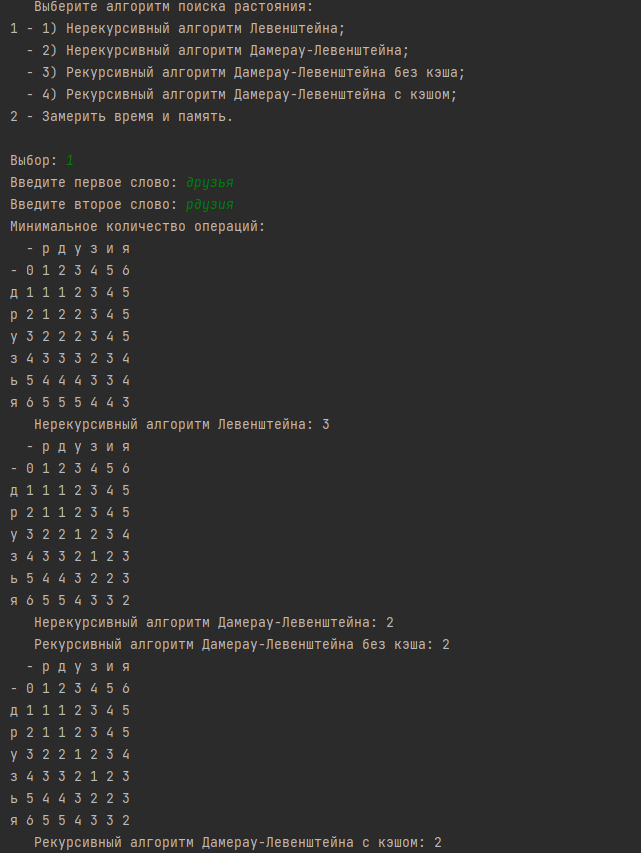
\includegraphics[height=0.4\textheight]{img/example.png}
	\caption{Демонстрация работы программы при поиске расстояние Левенштейна и Дамерау-Левенштейна}
	\label{img:demonstration}
\end{figure}

\clearpage

\section{Временные характеристики}

Результаты замеров по результатам экспериментов приведены в Таблице \ref{tbl:time}. В данной таблице для значений, для которых тестирование не выполнялось, в поле результата находится "\ - ".

\begin{table}[ht]
	\small
	\begin{center}
		\caption{Замер времени для строк, размером от 1 до 200}
		\label{tbl:time}
		\begin{tabular}{|c|c|c|c|c|}
			\hline
			& \multicolumn{4}{c|}{\bfseries Время, нс} \\ \cline{2-5}
			& \multicolumn{1}{c|}{\bfseries Левенштейн}
			& \multicolumn{3}{c|}{\bfseries Дамерау-Левенштейн} \\ \cline{2-5}
			\bfseries Длина (символ) & \bfseries Итеративный & \bfseries Итеративный & \multicolumn{2}{c|}{\bfseries Рекурсивный} \\ \cline{4-5}
			& & & \bfseries Без кэша & \bfseries С кэшом
			 \csvreader{csv/time.csv}{}
            {\\\hline \csvcoli & \csvcolii & \csvcoliii & \csvcoliv & \csvcolv} \\
			\hline
		\end{tabular}
	\end{center}
\end{table}

Отдельно сравним итеративные алгоритмы поиска расстояний Левенштейна и Дамерау--Левенштейна. Сравнение будет производится на основе данных, представленных в Таблице \ref{tbl:time}. Результат можно увидеть на Рисунке \ref{plt:time_01}.

При длинах строк менее 30 символов разница по времени между
итеративными реализациями незначительна, однако при увеличении длины
строки алгоритм поиска расстояния Левенштейна оказывается быстрее
вплоть до полутора раз (при длинах строк равных 200). Это обосновывается
тем, что у алгоритма поиска расстояния Дамерау-Левенштейна задействуется
дополнительная операция, которая замедляет алгоритм

\begin{figure}[h]
	\centering
	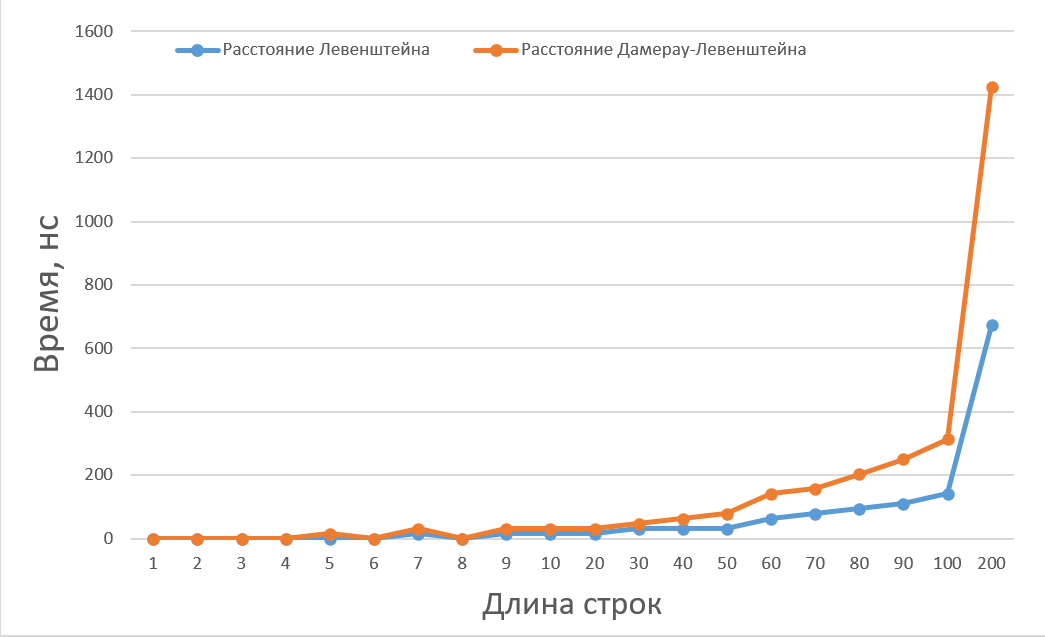
\includegraphics[height=0.3\textheight]{img/diag_01.png}
	\caption{Сравнение по времени алгоритмов поиска расстояния Левенштейн и Дамерау-Левенштейна -- нерекурсивной реализации}
	\label{plt:time_01}
\end{figure}

Так же сравним рекурсивную и итеративную реализации алгоритма поиска расстояния Дамерау-Левенштейна. Данные представлены в Таблице \ref{tbl:time} и отображены на Рисунке \ref{plt:time_02}.

\begin{figure}[h]
	\centering
	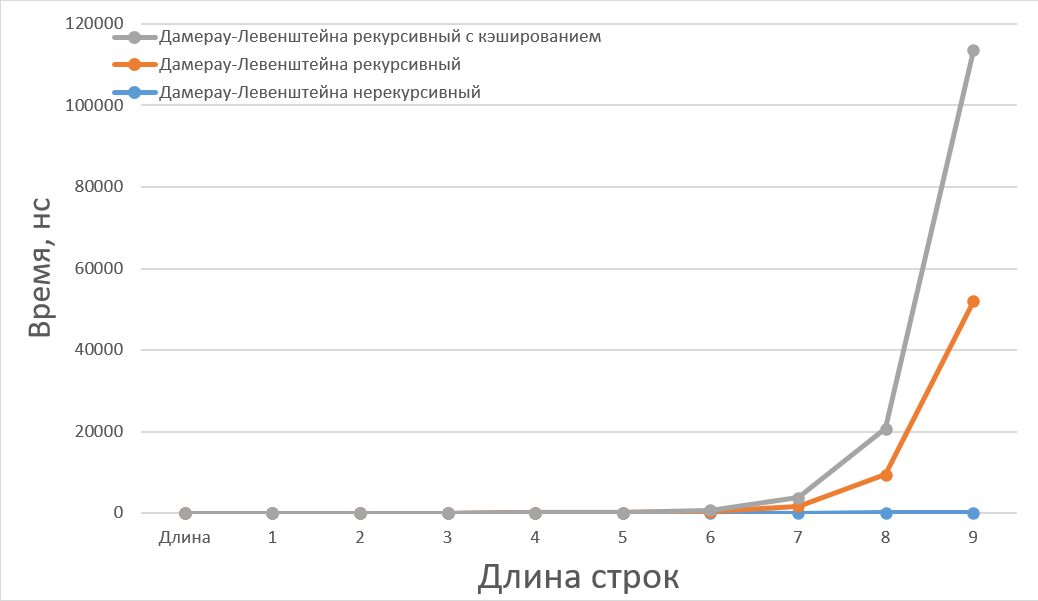
\includegraphics[height=0.3\textheight]{img/diag_02.png}
	\caption{Сравнение по времени алгоритмов поиска расстояния Дамерау-Левенштейна}
	\label{plt:time_02}
\end{figure}

На Рисунке \ref{plt:time_02} продемонстрировано, что рекурсивный алгоритм становится менее эффективным (вплоть до 21 раз при длине строк равной 7 элементов), чем итеративный.

Из этого можно сделать вывод о том, что при малых длинах строк (1-4 символа) предпочтительнее использовать рекурсивные алгоритмы, однако при обработке более длинных строк (болеее 3 символов) итеративные алгоритмы оказываются многократно более эффективными и рекомендованы к использованию.

Из данных, приведенных в  Таблице \ref{tbl:time}, видно, что итеративные алгоритмы становятся более эффективными по времени при увеличении длин строк, работая приблизительно в 308 млн. раз (Левенштейн) и 203 млн. раз (Дамерау-Левенштейн) быстрее, чем рекурсивные (при длинах строк равных 200). Однако, при малых длинах (1-4 элемента) рекурсивные алгоритмы работает по примерно как итеративные.

Кроме того, согласно данным, приведенным в Таблице \ref{tbl:time}, рекурсивные алгоритмы при длинах строк более 10 элементов не пригодны к использованию в силу экспоненциально роста затрат процессорного времени, в то время, как затраты итеративных алгоритмов по времени линейны.

\section{Характеристики по памяти}

Алгоритмы Левенштейна и Дамерау-Левенштейна не отличаются по использованию памяти, поэтому достаточно рассмотреть будет рассмотреть рекурсивную и матричную реализацию одного из этих алгоритмов.

Максимальная глубина стека вызовов при рекурсивной реализации равна сумме входящих строк, а на каждый вызов требуется 3 дополнительных переменных типа $integer$, соответственно, максимальный расход памяти

\begin{equation}
	(Len(S_{1}) + Len(S_{2})) \cdot (2 \cdot Size(\text{string}) + 5 \cdot Size(\text{int})),
\end{equation}
\noindent
где $S_{1}, S_{2}$ - строки, Size - функция, возвращающая размер аргумента; Len - функция, возвращающая длину строки, string - строковый тип, int - целочисленный.

Использование памяти при итеративной реализации теоретически равно:
\begin{equation}
	(Len(S_{1}) + 1) \cdot (Len(S_{2}) + 1) \cdot Size(int) + 3 \cdot Size(int) + 2 \cdot Size(string)
\end{equation}

По расходу памяти итеративные алгоритмы проигрывают рекурсивным: максимальный размер используемой памяти в них растёт как произведение длин строк, в то время как у рекурсивного алгоритма — как сумма длин строк.

\begin{table}[ht]
	\small
	\begin{center}
		\caption{Замер памяти для строк, размером от 10 до 200}
		\label{tbl:memory}
		\begin{tabular}{|c|c|c|}
			\hline
			& \multicolumn{2}{c|}{\bfseries Размер, байт} \\ \cline{2-3}
			\bfseries Длина (символ) & \bfseries Итеративный & \bfseries Рекурсивный
			 \csvreader{csv/memory.csv}{}
            {\\\hline \csvcoli & \csvcolii  & \csvcoliii} \\
			\hline
		\end{tabular}
	\end{center}
\end{table}

Из данных, приведенных в Таблице \ref{tbl:memory}, видно, что рекурсивные алгоритмы являются более эффективными по памяти, так как используется только память под локальные переменные, передаваемые аргументы и возвращаемое значение, в то время как итеративные алгоритмы затрачивают память линейно пропорционально длинам обрабатываемых строк.

В связи с этим, при недостаточном объеме памяти, рекомендуются использовать рекурсивные алгоритмы, так как они не используют дополнительной памяти в процессе работы.

\begin{figure}[h]
	\centering
	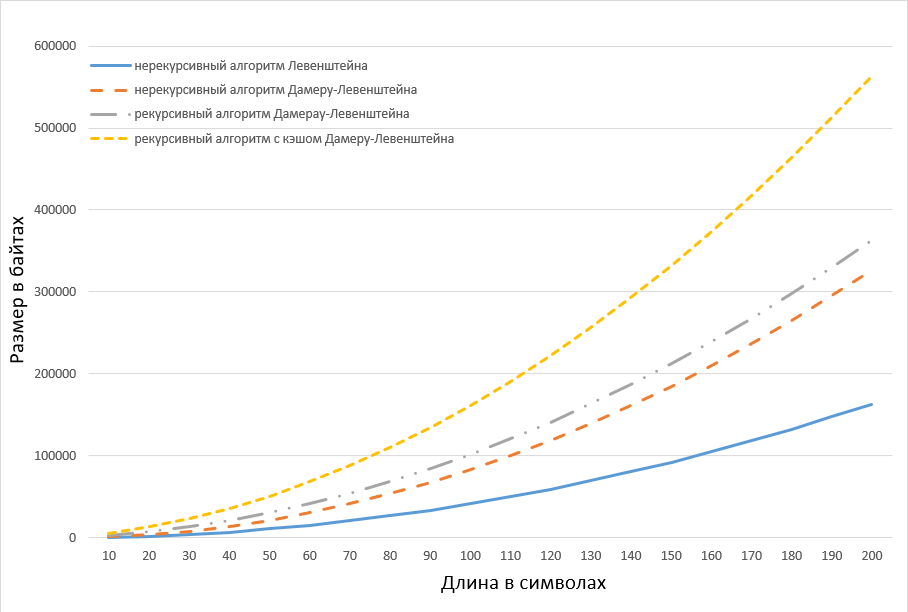
\includegraphics[height=0.3\textheight]{img/diag_03.png}
	\caption{Сравнение по памяти алгоритмов поиска расстояния Левенштейна и Дамерау-Левенштейна -- итеративной и рекурсивной реализации}
	\label{plt:memory_01}
\end{figure}

\begin{figure}[h]
	\centering
	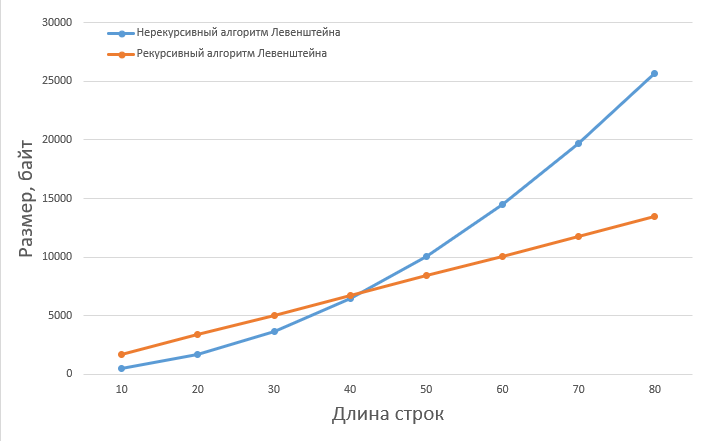
\includegraphics[height=0.3\textheight]{img/diag_04.png}
	\caption{Сравнение по памяти алгоритмов поиска расстояния Левенштейна и Дамерау-Левенштейна -- итеративной и рекурсивной реализации}
	\label{plt:memory_02}
\end{figure}

На Рисунке \ref{plt:memory_01} продемонстрировано, что итерационный алгоритм становится менее эффективным, чем рекурсивный если длина строк больше 40, достаточно хорошо это продемонстрировано на Рисунке \ref{plt:memory_02}.

\clearpage

\section{Сравнительный анализ алгоритмов}

Приведенные характеристики показывают нам, что рекурсивная реализация алгоритма очень сильно проигрывает по времени. В связи с этим, рекурсивные алгоритмы следует использовать лишь для малых размерностей строк (1-4 символа) или при малом объеме оперативной памяти.

Так как во время печати очень часто возникают ошибки связанные с транспозицией букв, алгоритм поиска расстояния Дамерау-Левенштейна является наиболее предпочтительным, не смотря на то, что он проигрывает по времени и памяти алгоритму Левенштейна.

Можно сделать вывод о том, что рекуррентный алгоритм поиска расстояния Дамерау-Левенштейна будет более затратным по времени по сравнению с итеративной реализацией алгоритма поиска расстояния Дамерау-Левенштейна.

\section{Вывод}
В данном разделе было произведено сравнение количества затраченного времени и памяти вышеизложенных алгоритмов. Наименее затратным по времени оказался рекурсивный алгоритм нахождения расстояния Дамерау-Левенштейна.

Для обработок малых длин строк (1-4 символа) предпочтительнее использовать рекурсивные алгоритмы, в то время как для остальных случаев рекомендуются использовать итеративные реализации. Однако, стоит учитывать дополнительные затраты по памяти, возникающие при использовании итеративных алгоритмов.

\chapter*{Заключение}
\addcontentsline{toc}{chapter}{Заключение}
Алгоритмы поиска расстояний Левенштейна и Дамерау-Левенштейна являются самыми популярными алгоритмами, которые помогают найти редакторское расстояние.

Поставленные цели работы были достигнуты и выполнены, т.е. в результате выполнения данной лабораторной работы были изучены алгоритмы поиска расстояний Левенштейна (Формула \ref{eq:L}) и Дамерау-Левенштейна (Формула \ref{eq:DL}), построены схемы (Рисунок \ref{fig:Liter}, Рисунок \ref{fig:ВLiter}), соответствующие данным алгоритмам, также разобраны рекурсивные алгоритмы (Рисунок \ref{fig:DLrec}, Рисунок \ref{fig:DLrechash1}). Реализован программный продукт, который вычисляет дистанцию 4 способами.

В рамках выполнения работы решены следующие задачи.
\begin{itemize}
	\item Изучены расстояния Левенштейна и Дамерау--Левенштейна.
	\item Реализованы алгоритмы поиска расстояний:
	\begin{itemize}
		\item Нерекурсивный алгоритм нахождения расстояния Левенштейна.
		\item Нерекурсивный алгоритм нахождения расстояния Дамерау-Левенштейна.
		\item Рекурсивный алгоритм нахождения расстояния Дамерау-Левенштейна.
		\item Рекурсивный алгоритм нахождения расстояния Дамерау-Левенштейна с кэшированием.
	\end{itemize}
	\item Замерено процессорное время работы реализаций алгоритмов поиска расстояний.
	\item Проведено сравнение временных характеристик, а также затраченной памяти.
\end{itemize}

\begin{thebibliography}{5}
	\bibitem{book_lev}
	Левенштейн В. И. Двоичные коды с исправлением выпадений, вставок и замещений символов. – М.: Доклады АН СССР, 1965. Т. 163. С. 845– 848.
	Режим доступа: \url{https://goo.su/8xIsL}
	\bibitem{cpp}
    Документация по Microsoft C++ [Электронный ресурс]. Режим доступа: \url{https://learn.microsoft.com/ru-ru/cpp/?view=msvc-170&viewFallbackFrom=vs-2017} (дата обращения: 25.09.2022).
	\bibitem{time}
	time — Time access and conversions [Электронный ресурс]. Режим доступа: \url{https://www.tutorialspoint.com/c_standard_library/c_function_clock.htm} (дата обращения: 25.09.2022).
	\bibitem{windows}
	Windows 10 Pro 2h21 64-bit  Электронный ресурс]. Режим доступа: \url{https://www.microsoft.com/ru-ru/software-download/windows10} (дата обращения: 25.09.2022).
	\bibitem{intel}
	Intel [Электронный ресурс]. Режим доступа: \url{https://ark.intel.com/content/www/ru/ru/ark/products/201839/intel-core-i510300h-processor-8m-cache-up-to-4-50-ghz.html} (дата обращения: 25.09.2022).
\end{thebibliography}

\addcontentsline{toc}{chapter}{Список литературы}

\end{document}